\documentclass[tikz, border=2pt]{standalone}
\usepackage{amsmath}

\begin{document}
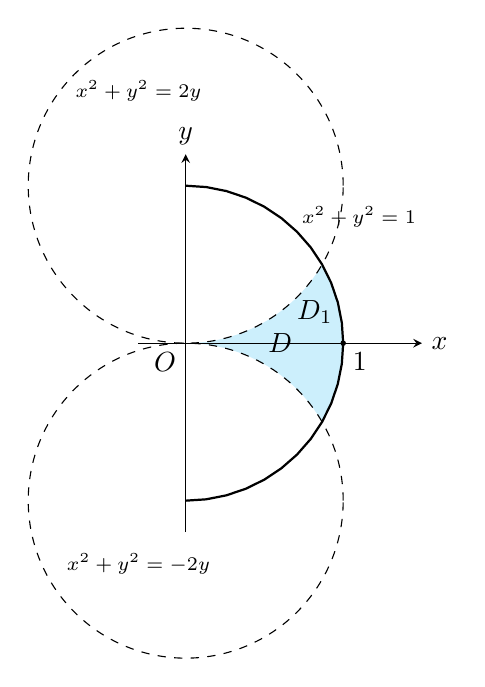
\begin{tikzpicture}[scale=2, >=stealth]
    % 填充积分区域 D
    % 路径说明：
    % 1. 从原点出发，沿上方小圆弧画到交点 (sqrt(3)/2, 0.5)
    % 2. 沿大圆弧画到下方交点 (sqrt(3)/2, -0.5)
    % 3. 沿下方小圆弧画回原点
    \fill[cyan!20] (0,0) arc (270:330:1) arc (30:-30:1) arc (30:90:1) -- cycle;

    % 画坐标轴
    \draw[->] (-0.3, 0) -- (1.5, 0) node[right] {$x$};
    \draw[->] (0, -1.2) -- (0, 1.2) node[above] {$y$};

    % 画大圆 x^2 + y^2 = 1 的右半部分
    \draw[thick, domain=-90:90] plot ({cos(\x)}, {sin(\x)});
    \node at (1.1, 0.8) {\scriptsize $x^2+y^2=1$};

    % 画上方小圆 x^2 + y^2 = 2y (即 x^2 + (y-1)^2 = 1)
    \draw[dashed, thin] (0,1) circle (1);
    \node at (-0.3, 1.6) {\scriptsize $x^2+y^2=2y$};

    % 画下方小圆 x^2 + y^2 = -2y (即 x^2 + (y+1)^2 = 1)
    \draw[dashed, thin] (0,-1) circle (1);
    \node at (-0.3, -1.4) {\scriptsize $x^2+y^2=-2y$};

    % 标注关键点
    \node[below left] at (0,0) {$O$};
    \fill (1,0) circle (0.5pt) node[below right] {$1$};

    % 标注区域 D
    \node at (0.6, 0) {$D$};
    \node at (0.82, 0.2) {$D_1$};
\end{tikzpicture}
\end{document}
